% To-dos
% ------
% - Figure 2: binned statistics for 3 potentials shown in Figure 1 showing statistics depend on angles
% - Figure 3: amplitude of cos(2theta) term vs. disk mass - show point and error-bar for zero-crossing
% - Figure 5: point and error-bar for different elements. Shaded band that represents the 1-sigma combination (invvar weighted) of the various tracers
% - Mean abundance deviation

\documentclass[modern]{aastex63}

\usepackage{xcolor}
\usepackage{amsmath}

\newcommand{\documentname}{\textsl{Article}}
\newcommand{\sectionname}{Section}
\renewcommand{\figurename}{Figure}
\newcommand{\equationname}{Equation}
\renewcommand{\tablename}{Table}

% Misc.
\newcommand{\bs}[1]{\boldsymbol{#1}}

% Missions
\newcommand{\project}[1]{\textsl{#1}}

% Packages / projects / programming
\newcommand{\package}[1]{\textsl{#1}}
\newcommand{\acronym}[1]{{\small{#1}}}
\newcommand{\github}{\package{GitHub}}
\newcommand{\python}{\package{Python}}

% Stats / probability
\newcommand{\given}{\,|\,}
\newcommand{\norm}{\mathcal{N}}
\newcommand{\pdf}{\textsl{pdf}}

% Maths
\newcommand{\dd}{\mathrm{d}}
\newcommand{\TT}[1]{\ensuremath{{#1}^{\mathsf{T}}}}
\newcommand{\transp}{\ensuremath{^{\mathsf{T}}}}
\newcommand{\inv}[1]{{#1}^{-1}}
\newcommand{\argmin}{\operatornamewithlimits{argmin}}
\newcommand{\mean}[1]{\left\langle #1 \right\rangle}

% Non-scalar variables
\renewcommand{\vec}[1]{\ensuremath{\bs{#1}}}
\newcommand{\mat}[1]{\ensuremath{\mathbf{#1}}}

% Unit shortcuts
\newcommand{\Msun}{\ensuremath{\mathrm{M}_\odot}}
\newcommand{\Mjup}{\ensuremath{\mathrm{M}_{\mathrm{J}}}}
\newcommand{\kms}{\ensuremath{\mathrm{km}~\mathrm{s}^{-1}}}
\newcommand{\mps}{\ensuremath{\mathrm{m}~\mathrm{s}^{-1}}}
\newcommand{\pc}{\ensuremath{\mathrm{pc}}}
\newcommand{\kpc}{\ensuremath{\mathrm{kpc}}}
\newcommand{\kmskpc}{\ensuremath{\mathrm{km}~\mathrm{s}^{-1}~\mathrm{kpc}^{-1}}}
\newcommand{\dayd}{\ensuremath{\mathrm{d}}}
\newcommand{\yr}{\ensuremath{\mathrm{yr}}}
\newcommand{\AU}{\ensuremath{\mathrm{AU}}}
\newcommand{\Kel}{\ensuremath{\mathrm{K}}}
\newcommand{\mas}{\ensuremath{\mathrm{mas}}}

% Astronomy
\newcommand{\DM}{{\rm DM}}
\newcommand{\abunratio}[2]{\ensuremath{{[\mathrm{#1}/\mathrm{#2}]}}}
\newcommand{\feh}{\abunratio{Fe}{H}}
\newcommand{\mh}{\abunratio{M}{H}}
\newcommand{\alphafe}{\abunratio{\alpha}{Fe}}
\newcommand{\mgfe}{\abunratio{Mg}{Fe}}
\newcommand{\df}{\acronym{DF}}
\newcommand{\logg}{\ensuremath{\log g}}
\newcommand{\Teff}{\ensuremath{T_{\textrm{eff}}}}
\newcommand{\mtwomin}{\ensuremath{M_{2, {\rm min}}}}

% Colors:
\definecolor{tabblue}{HTML}{4E79A7}
\definecolor{taborange}{HTML}{F28E2B}
\definecolor{tabgreen}{HTML}{59A14F}
\definecolor{tabred}{HTML}{E15759}
\definecolor{tabpurple}{HTML}{B07AA1}

% TODO:
\newcommand{\TODO}[1]{{\color{tabgreen}\textbf{TODO:} #1}}
\newcommand{\APWTODO}[1]{{\color{tabpurple}\textbf{APW TODO:} #1}}
\newcommand{\HOGGTODO}[1]{{\color{tabred}\textbf{HOGG TODO:} #1}}


% text macros
\newcommand{\methodname}{\textsl{Abundance Torus Method}}
% Torus Tomography
%   Torus Topography (see what I did there?)
% Abundance-Moment foliation (AMF)
%   Abundance-Moment laminae (AML)
% Abundance Torus Machinery (ATM)
%   Abundance Torus Method (ATM)
%   Abundance Torus
% Toroidal abundance blender (TAB)
%   Toroidal abundance mixer (or mixmaster) (TAM)
% Stationary Abundance Tori (SAT)
%   Stationary Abundance Torus Method (SATM)
% Chemical Tangents
%   Abundance Tangent Method (ATM)
%   Compositional Tangents
% Composition Gradient Method (CGM)
% Abundance Isopleth Method (AIM)
% The Magical 3-torus of Invariance (MTI)
% \newcommand{\method}{\acronym{TMR}}

% Project-specific macros - all others go in preamble.tex
\newcommand{\gaia}{\textsl{Gaia}}
\newcommand{\dr}[1]{\acronym{DR}#1}
\newcommand{\apogee}{\acronym{APOGEE}}
\newcommand{\sdss}{\acronym{SDSS}}
\newcommand{\sdssiv}{\acronym{SDSS-IV}}
\newcommand{\sdssv}{\acronym{SDSS-V}}
\newcommand{\galah}{\acronym{GALAH}}
\newcommand{\hermes}{\acronym{HERMES}}

\setlength{\parindent}{1.1\baselineskip} % trust in Hogg
\shorttitle{tags are separable from angles}
\shortauthors{Price-Whelan et al.}

\begin{document}\sloppy\sloppypar\raggedbottom\frenchspacing % trust in Hogg
\graphicspath{ {figures/} }
\DeclareGraphicsExtensions{.pdf,.eps,.png}

\title{\textbf{%
    Revealing the orbital foliation of phase space\\
    through invariances of element-abundance distributions}}

\newcommand{\affcca}{Center for Computational Astrophysics, Flatiron Institute, 162 Fifth Ave, New York, NY 10010, USA}
\newcommand{\affccpp}{Center for Cosmology and Particle Physics, Department of Physics, New York University, 726 Broadway, New York, NY 10003, USA}
\newcommand{\affmpia}{Max-Planck-Institut f\"ur Astronomie, K\"onigstuhl 17, D-69117 Heidelberg, Germany}
\newcommand{\affcolumbia}{Department of Astronomy, Columbia University, New York, NY 10027, USA}

\author[0000-0003-0872-7098]{Adrian~M.~Price-Whelan}
\affiliation{\affcca}

\author[0000-0003-2866-9403]{David~W.~Hogg}
\affiliation{\affcca}
\affiliation{\affmpia}
\affiliation{\affccpp}

\author[0000-0001-6244-6727]{Kathryn~V.~Johnston}
\affiliation{\affcca}
\affiliation{\affcolumbia}

\author[0000-0003-4996-9069]{Hans-Walter~Rix}
\affiliation{\affmpia}

\author{others}

\begin{abstract}\noindent
  The dynamics of stars in the Milky Way and nearby galaxies is often
  interpreted in an approximation where the gravitational potential is treated
  as simple and integrable and the distribution function time-invariant.
  Under these conditions, Jeans modeling---which relies on computing and
  observing moments of the distribution function---is a standard methodology for
  measuring properties of the mass distribution or potential.
  However, contemporary and near-future spectroscopic surveys measure more than
  just kinematics for huge samples of individual stars within the Milky Way and
  local group.
  Here we present an approach for dynamical
  inference---\methodname---that makes use of kinematic measurements
  and \emph{stellar tags} (e.g., element abundances, stellar ages, or other
  invariant stellar properties).
  The method exploits the fact that there are generically gradients of stellar
  tags on position and velocity in the Galaxy:
  In steady state, the distributions of any tags must be invariant with respect
  to time-variable conjugate angles.
  Thus, level sets in moments of the tag distributions must coincide with
  the orbital foliation of phase space!
  We discuss how both classical-statistics and Bayesian forward-modeling methods
  can be built on this idea, and we perform a demonstration with red giant
  stars from the \apogee\ surveys:
  We look at vertical orbit structure in the
  Milky Way disk, using mean abundance to constrain the local disk mass (the disk--halo
  trade-off at fixed circular velocity).
  We find that the disk mass can be constrained na\"ively at the $<10$-percent
  level with this new method using only a single moment of a single element
  abundance, demonstrating the promise of combining stellar tags with
  dynamical invariants.
\end{abstract}

\keywords{\raggedright % now from the UAT, not the AAS keyword system
  astrometry
  ---
  astrostatistics
  ---
  chemical~abundances % UGH ELEMENTS
  ---
  galaxy~dynamics
  ---
  Milky~Way~dynamics
  ---
  radial~velocity
  ---
  spectroscopy
  ---
  stellar~kinematics
  ---
  surveys
}

% \section*{}\clearpage
\section{Introduction}

Physicists of the 18th century worked out that the gravitational force
law in the Solar System is proportional to the inverse square of the
distance from the Sun (CITE Newton).
That inference was based on the observation that orbits in the Solar
System are closed ellipses (CITE Kepler).
We physicists of the 21st century are trying to work out the map of
gravitational acceleration (or gravitational
potential, or mass distribution) in the Milky Way.
We are at a disadvantage, in some sense, because no-one gets to see
the orbits of stars in the Milky Way: Even in the whole history of
western science, stars have barely moved in Galactic coordinates.
The tools we use generally ask statistical questions about velocity
moments (CITE Jeans and Oort and B\&T); we never see the orbits directly.
The closest we come to seeing orbits directly in the Milky Way is in the
study of stellar streams (CITE), but these are rare and mainly exist at large
Galactocentric distances.

Okay fine, really we are at a \emph{huge advantage} with respect to
our 18th century counterparts, because we have a very accurate theory
of gravity (CITE), an excellent working model of stars (CITE),
and immense observational and computational resources.
With these resources we have measured the element abundances of the
stellar photospheres of hundreds of thousands of stars (CITE) and
precise positions and velocities of millions.
In this \documentname\ we are going to demonstrate that these
measurements can be used to illuminate the orbit structure in the
Milky Way, even---or especially---in the dense, nearby parts of the
disk.
Our method will work only under strong assumptions, so we are
still in the business of revealing the orbits indirectly.
However, our approach is novel and there are many regimes in which it
will be more precise than any other method.

In a well-mixed population, stars are in a kinematic steady state:
As time goes on, stars move along their orbits, but they don't change their dynamical
invariants (by assumption!) and every location in angle (and by ``angle'' we mean the
coordinate conjugate to action in action--angle coordinates) is equally likely, or
equally probably populated in any snapshot.
The chemical-tagging insight (CITE) is that the stars also don't change
their surface element abundances as they orbit.
That is, in an integrable galaxy---a galaxy whose gravitational orbits
are associated with three invariant actions---the element abundances and
the dynamical actions have something in common:
They don't change with time.
Only the conjugate angles, conjugate to those actions, do.
This means that, for a well-mixed population, the detailed element abundances can only
be a function of actions, and never a function of conjugate angles.
That's a remarkably informative constraint on the configuration of the Milky Way in
the space of positions (3), velocities (3), and detailed abundances (10 to 30, depending
on survey).

Consider a collection of stars (localized, say, in phase space) for which we have
measured $D$ element abundances.
This collection of stars will in general have a diversity of element abundances.
That is, their abundances are drawn from some density or distribution or pdf in
$D$-dimensional element-abundance space.
Now consider how this abundance distribution varies as we move around in phase space.
It will vary in general (there are radial and vertical abundance gradients in the
disk, for example).
Any gradient we observe in these element-abundance distributions with respect to
phase-space coordinates (that is, the six-gradient) must not project
onto the directions of increasing (or decreasing) conjugate angles in phase space.
That is, all gradients with respect to phase-space coordinates
of the element-abundance distribution must be orthogonal to the
directions of increase (or decrease) of the conjugate angles, and lie in the subspace
of the directions of increase (or decrease) of the dynamical actions.
The trajectories of stars in the phase space (the dynamical tori) must lie along or
describe level surfaces in the element-abundance distribution!

% Notebook: figures/APOGEE-zvz-orbits.ipynb
\begin{figure}[!tp]
  \begin{center}
  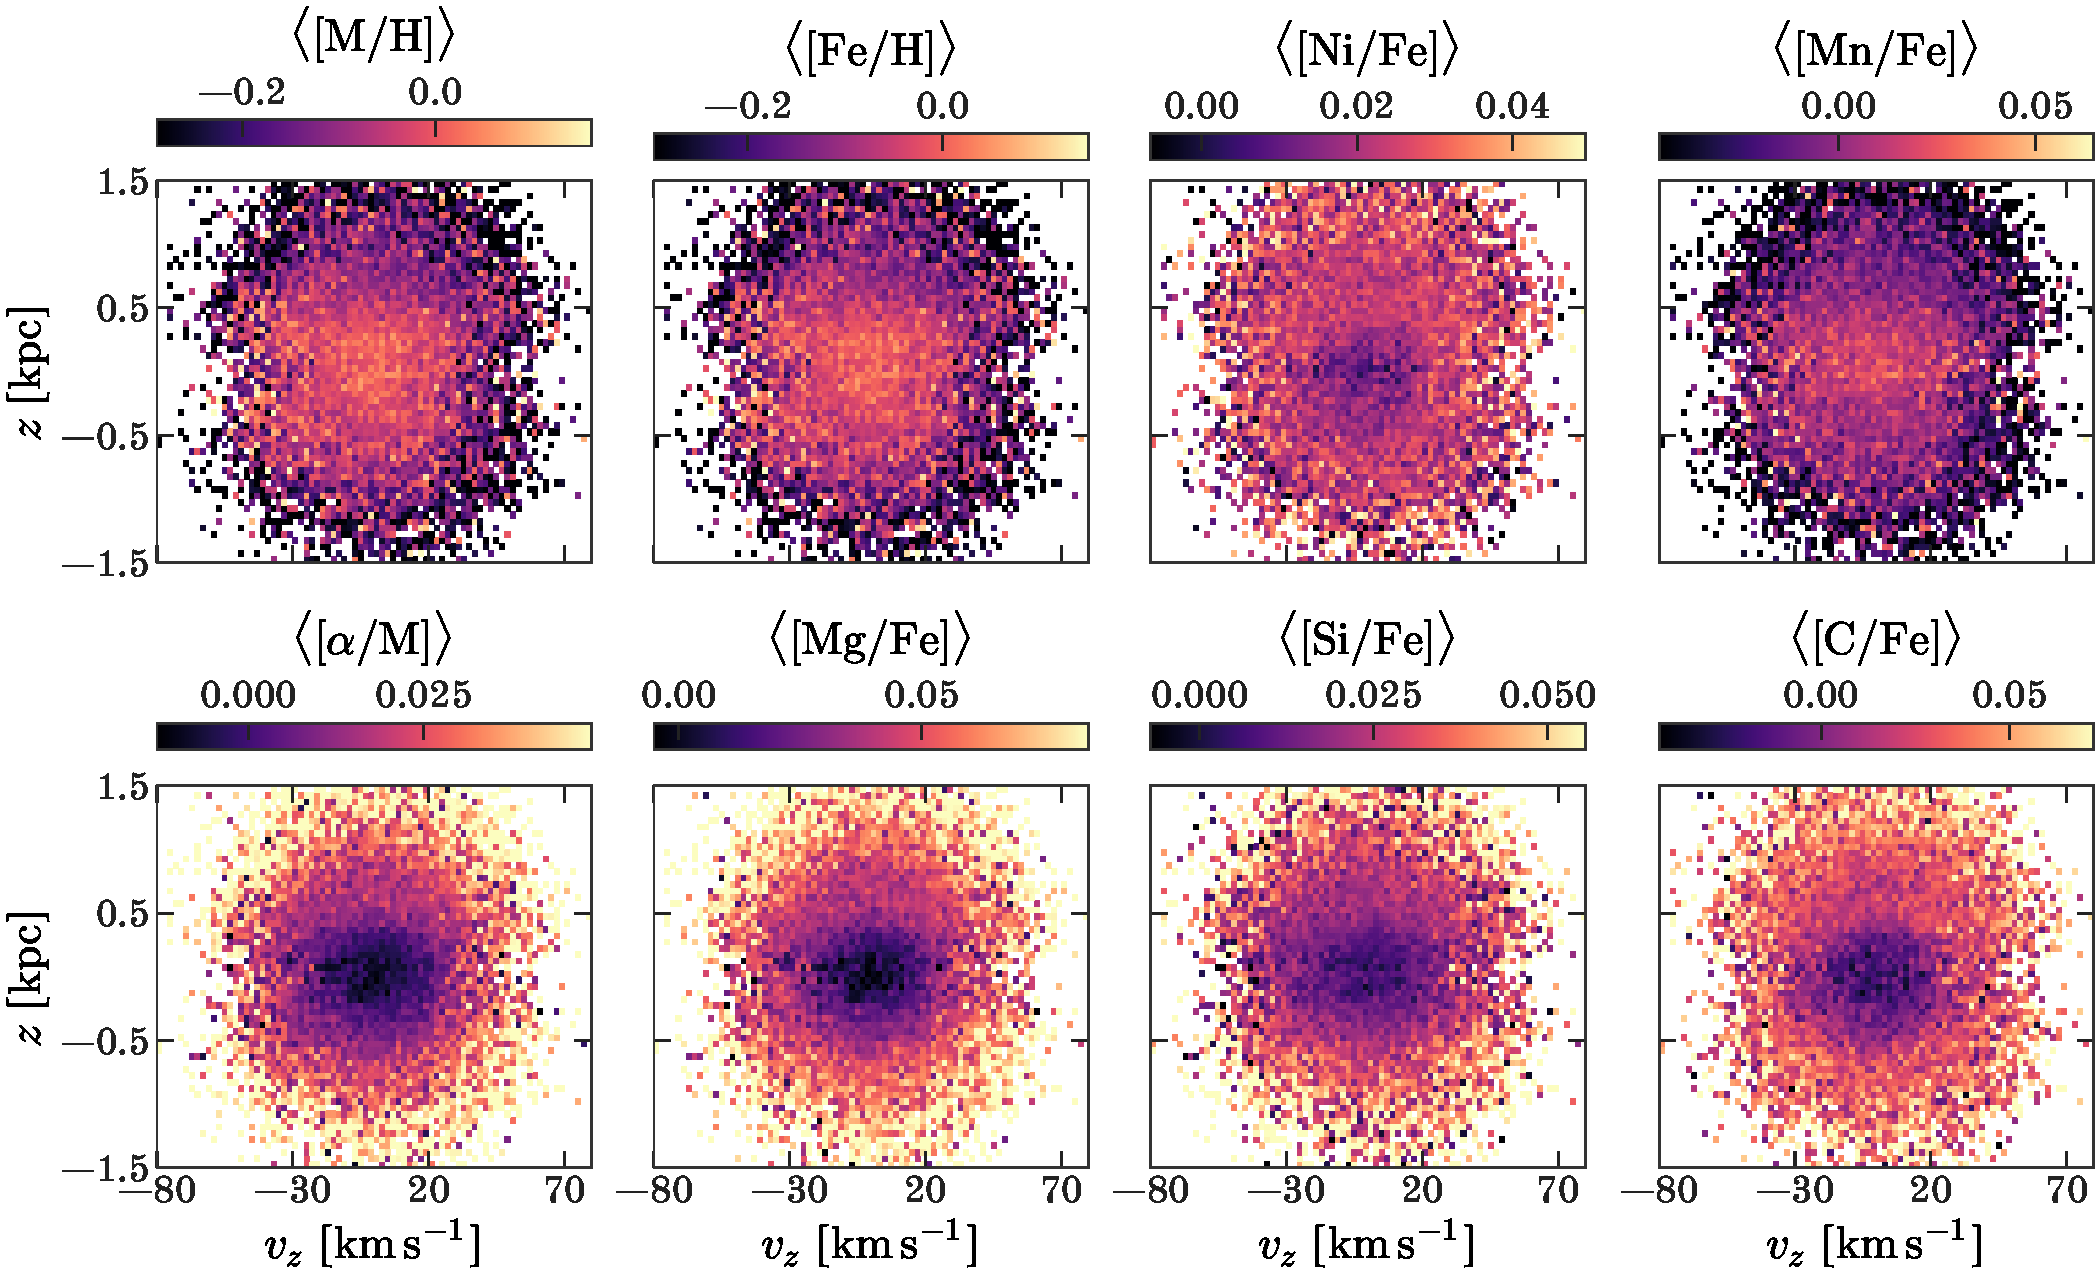
\includegraphics[width=\textwidth]{abundance-zvz-grid.pdf}
  \end{center}
  \caption{%
    The means of various (logarithmic) abundance ratios as a function of
    Galactic vertical height $z$ and vertical velocity $v_z$.
    Averages are taken in $z, v_z$ boxels.
    The stars at lower $|z|$ and lower $|v_z|$ (that is, the stars with
    lower overall vertical action $J_z$) show higher overall metallicity
    on average, but lower alpha-to-iron.
    These plots are somewhat affected by \apogee\ selection effects, in
    that different $z, v_z$ boxels are projections through different extents
    in Galactocentric radius. This explains some of the visible asymmetries.
  \label{fig:zvz-grid}
  }
\end{figure}

% Notebook: figures/zvz-orbit-demo.ipynb
\begin{figure}[!tp]
  \begin{center}
  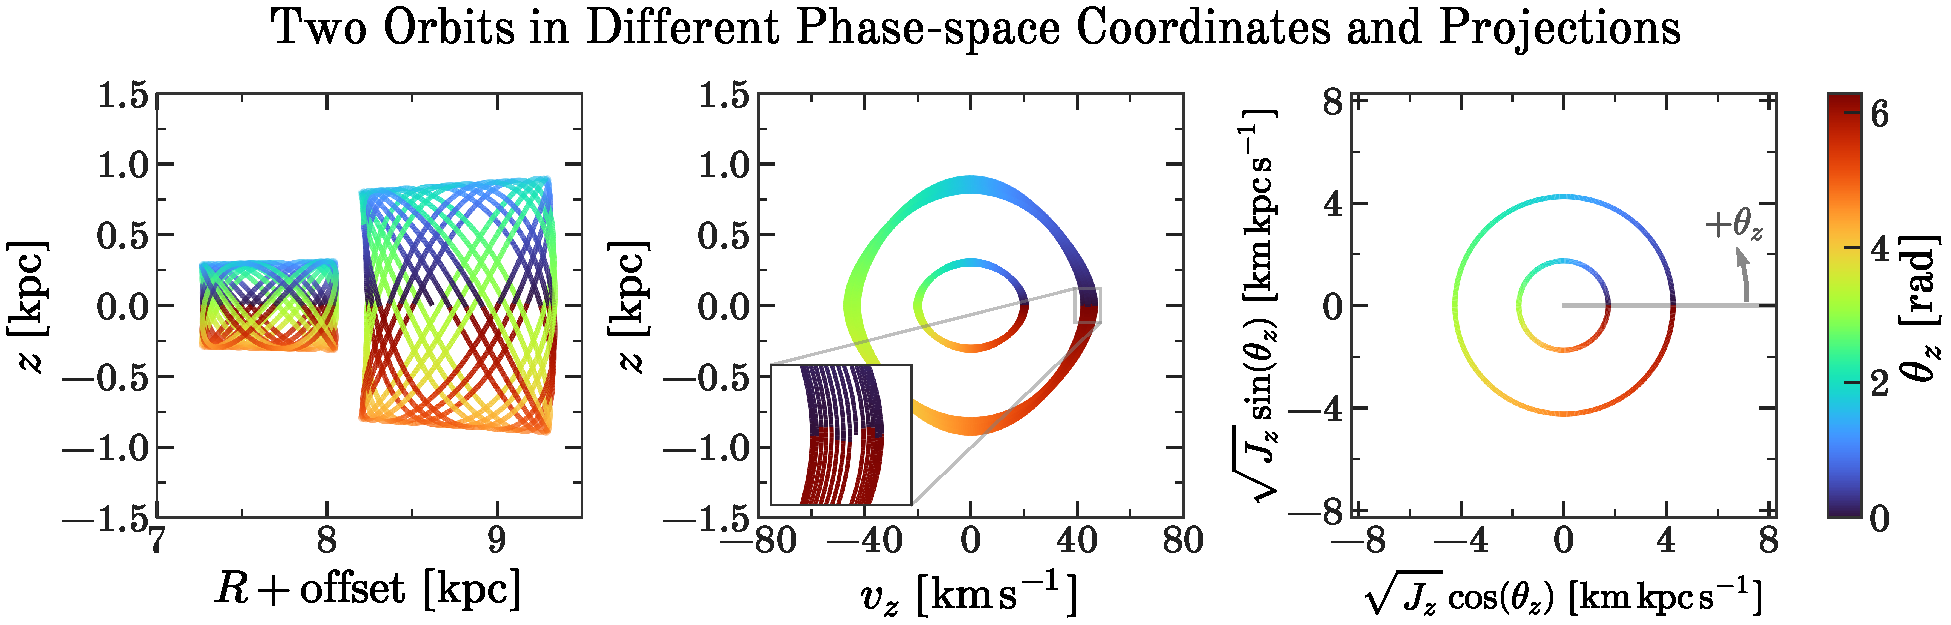
\includegraphics[width=\textwidth]{zvz-orbit-demo.pdf}
  \end{center}
  \caption{%
    \textsl{Left panel:} Two orbits projected onto the plane of
    Galactic vertical height $z$ and Galactocentric cylindrical radius
    $R$. The orbits fill the surfaces of 3-tori in 6-d phase space.
    \textsl{Middle panel:} The same two orbits, but projected onto the plane
    of vertical height $z$ and vertical velocity $v_z$. In this projection,
    it becomes clearer that the orbital lines are
    colored by the angle $\theta_z$ that is conjugate to vertical action $J_z$.
    The inset shows that conjugate angle wraps non-trivially, because the action
    (by construction) wraps at constant angular velocity, whereas the vertical period
    is a (weak) function of the other orbital phases.
    Note that although this projection is close to ``face on'' for these two
    orbits, the fact that they fills the surfaces of 3-tori means that they
    project to finite-width bands in $z, v_z$ space.
    \textsl{Right panel:} The same two orbits, but now plotted in vertical-action,
    vertical-angle space. In this space, the two orbits trace perfect circles.
    APW: THE FIGURE IS CUT OFF ON THE LEFT. ALSO ZOOM IN THE RIGHT PANEL SLIGHTLY MORE.
  \label{fig:zvz-demo}
  }
\end{figure}

% Notebook: figures/APOGEE-zvz-orbits.ipynb
\begin{figure}[!tp]
  \begin{center}
  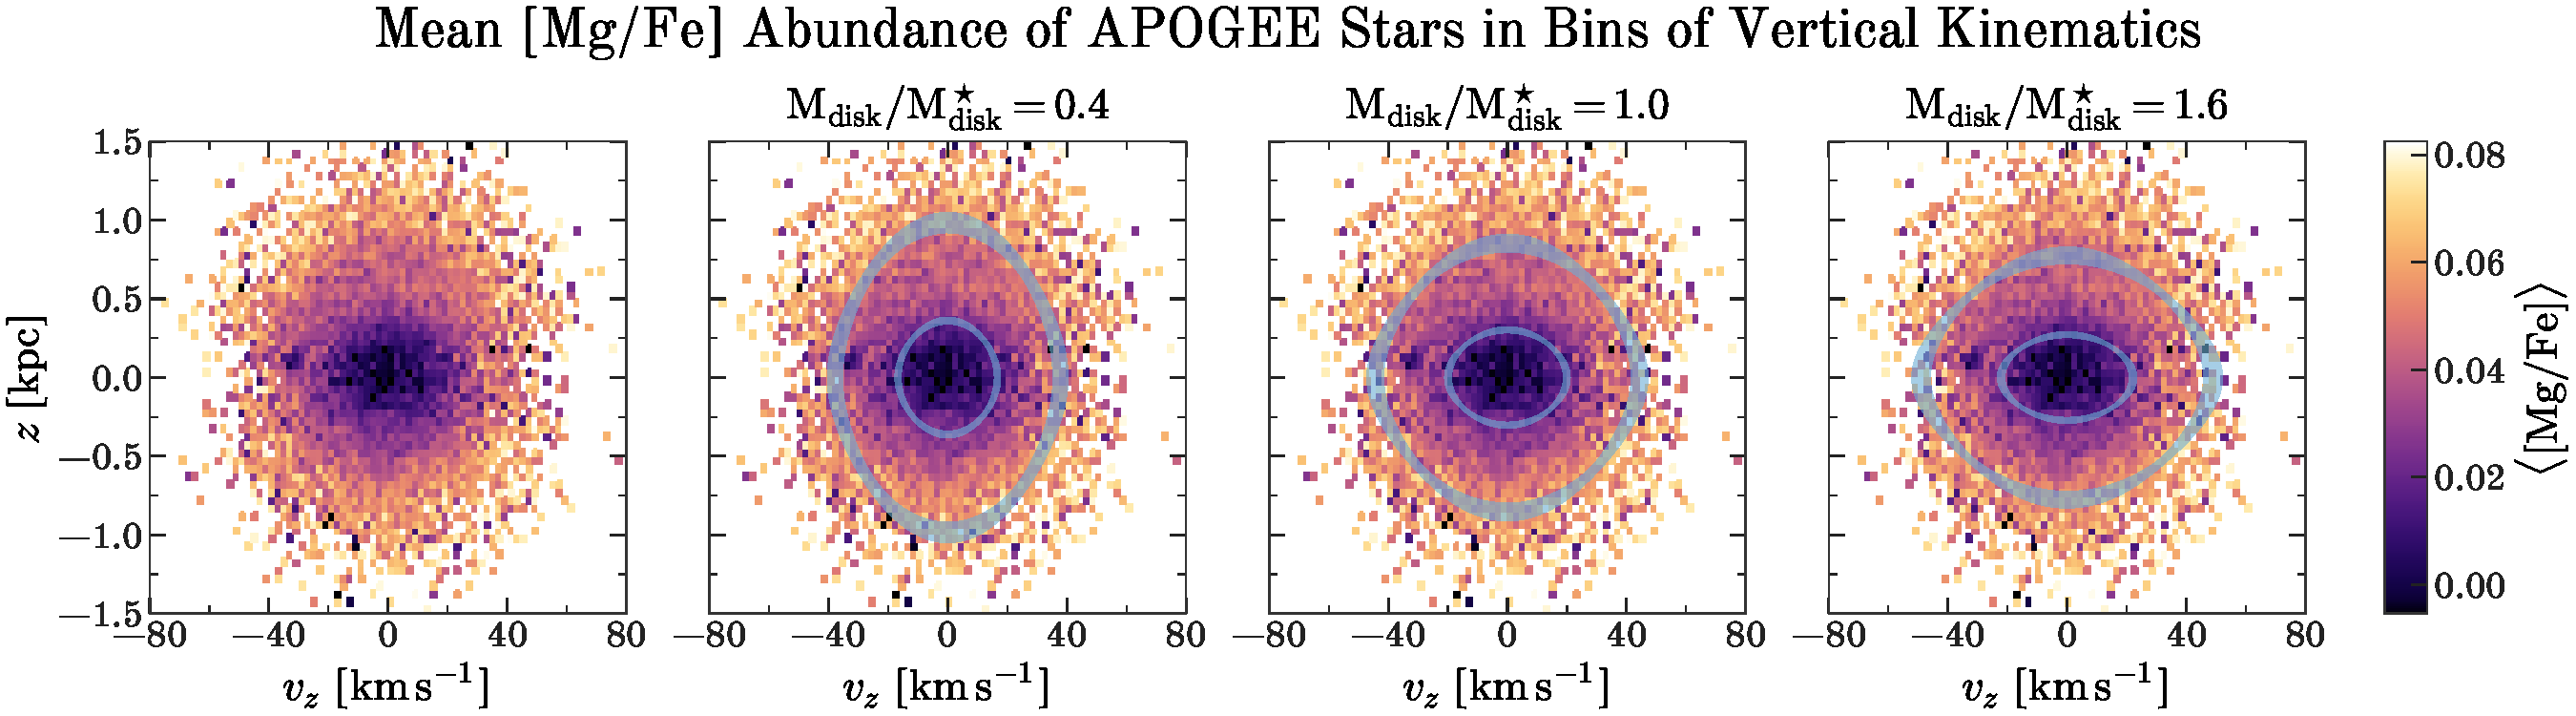
\includegraphics[width=\textwidth]{zvz-mean-MG_FE}
  \end{center}
  \caption{%
    \textsl{Left panel:} Repeat of the $\mgfe$ panel of \figurename~\ref{fig:zvz-grid}.
    \textsl{Other panels:} Same as the left panel, but with the two orbits
    from \figurename~\ref{fig:zvz-demo}
    over-plotted, for three different Milky Way potentials.
    These three potentials have the fiducial Milky Way disk mass (see text
    for details), or a disk less massive by a factor of 0.4 or more
    massive by a factor of 1.6, as noted in each panel title.
    All potentials are constrained to have a circular velocity at the
    Solar circle of $229\,\kms$.
    \emph{Which of the three panels appears most like the orbits are
    coincident with isopleths of the mean abundance?}
    This question is asked for illustrative purposes only: These
    plots distort the data by projection in phase space.
    In the methods used for the inferences we perform in
    \sectionname~XXX, all averages are performed in tiny
    three-dimensional action neighborhoods; we don't project the data in this way.
  \label{fig:zvz-mgfe}
  }
\end{figure}

WE WILL DEMONSTRATE WITH JUST VERTICAL KINEMATICS, BUT WE ARE NOT
GOING TO ASSUME SEPARABILITY.  Jeans models can suck it.

\section{Methodological generalities}

This project---\methodname---was motivated by plots of abundances of stars as a
function of vertical height $z$ and vertical velocity $v_z$ in
Galactocentric cylindrical coordinates, colored by element abundances.
Examples are shown in \figurename~\ref{fig:zvz-grid}.
In these plots,
the eye is drawn to \emph{abundance gradients}: The stars at small
heights and small vertical velocities have different abundance ratios,
on average, than stars at large heights and large vertical velocities.
But these positional and velocity gradients are related:
Stars at large absolute vertical velocities $v_z$ will, in the future, at some
times be at large absolute vertical positions $z$ (far from the plane, that is),
and stars at large absolute vertical positions will, in the future,
at some times be at large absolute vertical velocities.
That is, the stars will orbit in the Galaxy.
And stars don't---to very high precision---change their abundances as
they orbit.

One consequence of these observations is a new method for inferring
the orbit structure of the Milky Way:
If two small neighborhoods in phase space lie on the same orbit---that
is, they correspond to the same dynamical actions or they can be reached
by common initial conditions---they must contain stars with the same distribution of
element abundances.
This prediction depends on many detailed assumptions, such as that
the Galaxy is (approximately) phase mixed, and that the potential is
(approximately) time invariant and integrable.
And of course the \emph{usefulness} of this prediction for inference
depends on the existence of gradients: If there aren't
element-abundance-ratio gradients, there will be no information to work
with.
There are many ways to describe the fundamental prediction that underlies \methodname.
Here are a few:
\begin{itemize}
\item
  Stars don't change their abundances as they orbit!  Stellar
  abundance ratios can depend on the three invariant actions, but they
  can't depend on the conjugate angles, which wind up arbitrarily with time.
  This can be seen as a kinematic description of the concept underlying this \documentname.
\item
  Or, equivalently, abundance gradients taken in 6-dimensional phase space will be
  locally perpendicular, everywhere, to the orbital 3-tori in phase space.
  This is a local-geometry description of the concept.
\item
  Or, equivalently, at every location in 6-d phase space, there are a set of 6-d
  gradient vectors, which are the derivatives of all measurable
  moments of all measurable element-abundance ratios with respect to
  the 6 phase-space coordinates. These gradient vectors will span a
  local 3-d subspace, and this subspace will be orthogonal to the surfaces
  of the orbital tori at that location.
  This is a mathematics-of-gradients description.
\item
  Or, equivalently, the orbital tori will be level 3-surfaces in 6-d phase space of any
  moments or statistics of the element-abundance distribution.
  This is a global-geometry description.
\item
  Or, equivalently, a predictive model for the element abundances of stars
  that is given the freedom to depend on both actions and angles will do no
  better at predicting stellar element abundances than a model that is only
  given the freedom to depend on actions alone.
  This is an information-theory description.
\end{itemize}

The points are illustrated graphically in \figurename~\ref{fig:zvz-mgfe}:
In the fiducial model, the two overlaid orbits more-or-less follow something
like a mean abundance contour.
In the model in which the disk is made less massive (and the halo more massive
to keep the circular velocity constant), the orbits change shape: There is more
positional extent to an orbit relative to it's velocity extent.
The orbital frequency $\omega$ is, to order of magnitude, the velocity amplitude
divided by the spatial amplitude, and it is, to order of magnitude, $\sqrt{G\,\rho}$,
where $\rho$ is the mean enclosed mass density.
If stars were traveling on these lower-disk-mass orbits, they would have to
obtain higher abundances when they are passing through the disk midplane,
and lower abundances when they are at their greatest absolute vertical heights,
which is absurd: Stars do not change their abundances as they orbit.

We make this point clear in a different way in \figurename~YYY, in which
we have transformed into action--angle coordinates in phase space (CITE)
and we show scatterplots of the abundances as a function of conjugate
angles $\theta_z$, conjugate to the vertical actions $J_z$, for stars near
the orbits plotted in \figurename~XXX.
Using the fiducial potential to convert to actions and angles,
the abundance distribution is similar at different
angles $\theta_z$, or on different parts of the orbit.
Along the orbits generated by the low-mass-disk and high-mass-disk potentials,
the abundance distribution shows clear $m=2$ (or $\exp i\,2\,\theta_z$) dependences
on vertical angle $\theta_z$.
That is, just by plotting the abundances versus angle, we can make
inferences about the mass of the disk, or---more generally---the
gravitational potential of the Milky Way.

In order to make the abundance--angle plots in \figurename~YYY, we had
to DO SOME THINGS because we needed to visualize the global dependence
on angle using all the stars on all different kinds of orbits.
Because different orbits have different abundance-ratio
distributions, this is not a trivial transformation of the data.
In the inferences we do in \sectionname~AAA below, we
will use regression (frequentist) or forward modeling (Bayes) to
combine the data from stars on different orbits.

...The point that this works at one to three dimensions. It requires
abundance gradients, but not separability!  Of course you might not
have abundance gradients in all three action directions.

...The point that the method is combinatoric in abundance data.
...
One of the crazy things about all this is that any description of a general distribution in $D$-space
requires a \emph{lot of parameters}.
Even a trivial distribution---the Normal distribution---requires $0.5\,D\,(D+3)$ parameters for its
complete description, and anything more complex has more.
That means that there are a very large set of element-abundance statistics for which the
six-gradient exists or could be constraining for this project.
Not all of these parameters can be reliably measured in a finite data set,
let alone reliably seen to vary with phase-space location.
However, we choose to see this bug as a feature:
We have discovered, in effect, a \emph{combinatorically large set of constraints on the
dynamical actions and conjugate angles}.

...The point that this would be more complex in chaotic regions, and
maybe effectively inapplicable?

...The point that this doesn't depend on selection, provided that
stellar properties don't vary strongly with abundnaces, and that
abundance-measurement biases don't depend strongly on stellar
parameters. Both assumptions wrong in detail.

... The point that there will be frequentist statistics or
optimizations, and also Bayesian approaches.  The point that Bayes and
frequentism look very different here. Call out to orbital roulette,
and to Bovy et al.

In what follows, a very limited project...

\section{Data}

We use spectroscopic data from data release 16 (\dr{16}) of the \apogee\ surveys
(\citealt{Majewski:2017, DR16}; J\"onsson et al., in prep.).
\apogee\ is a component of the Sloan Digital Sky Survey IV (\sdssiv;
\citealt{Gunn:2006, Blanton:2017}); its main goal is to survey the chemical
and dynamical properties of stars across much of the Milky Way disk by obtaining
high-resolution ($R \sim 22,500$; \citealt{Wilson:2019}), infrared ($H$-band)
spectroscopy of hundreds of thousands of stars.
The primary survey targets are selected with simple color and magnitude cuts
\citep{Zasowski:2013, Zasowski:2017}, but the survey uses fiber-plugged plates
that cover only a small fraction of the available area, which leads to extremely
nonuniform coverage of the Galactic stellar distribution (see, e.g., Figure~1 in
\citealt{DR16}).


HOGG SAY: This section is APW's problem (ish).

APW: \apogee\ bread-and-butter and citations.

APW: Removal of stellar clusters from the data.

APW: Distance estimation.

APW: Choice of abundances.

APW: Final data properties (and possibly figures).

\section{Milky Way mass model and actions}

HOGG SAY: Possible section for APW to put details of the Milky Way model,
how we parameterize the disk mass, and how we compute actions and angles.
Or, if there isn't much to say, this can be part of the inferences section
below.

This section could describe our one mass-model parameter, and show how
the mass distribution and orbit structure vary as we vary it.

This section could also describe all the computational tips and tricks.

\section{Assumptions}

\methodname flows from a specific set of assumptions.
That is, we are going to make hard (and sometimes controversial) assumptions.
Our position is not that these assumptions are correct.
Our position is that our
methods are conditionally correct, conditioning on these assumptions.
\begin{description}
\item[integrable] HOGG: There are 3 invariants and 3 angles. This could perhaps be
  relaxed, but we don't know how yet.

\item[well mixed] HOGG: All angles equally likely.
  The well-mixed assumption will be violated substantially in the data;
  we will discuss this more below. But this is the fundamental assumption of
  the vast majority of inferences of the Milky Way mass distribution.

\item[selection] HOGG: Selection depends on position in the Milky Way, but not
  on element abundances. Really it could even depend on velocity! But it can't depend
  on abundances. That might be very slightly wrong.

\item[kinematic measurements] HOGG: Very strong assumption that phase space positions
  in 6-d are accurate and precise. So precise we don't have to generate them, we can
  condition on them!

\item[abundance measurements] HOGG: Assumption that stars in different parts of phase
  space get the same abundance measurements. Questionable in certain kinds of samples.
  HOGG: Oddly I don't think we need to assume that the chemical measurements have good
  (or any) noise estimates. They could be terrible, I think.

\item[smooth gradients] HOGG: Assumption about how the abundances can
  depend on action. Relatedly, the use of action and not log-action
  or zmax or whatever.
\end{description}

\section{Inferences}

HOGG: There are two approaches, with very different appearances, but
embodying the same fundamental assumptions.

HOGG: discriminative methods: frequentist forms; About finding the mass model in which
there is no residual dependence of abundance distributions on angles.
Technically these models are not strictly ``discriminative'' but it is a related
concept. Oh wait, I could truly make a discriminative model...

HOGG: generative methods: frequentist or Bayesian forms; About generating the abundances
with a model using only Actions.

HOGG: How are these qualitatively different methods related?

HOGG: Get more specific about forms and math.

HOGG: Show results on the data.

\section{Relationship to Jeans and other methods}

HOGG ASKS: What to write here? How detailed should we be? Or should this just
go to the discussion section?

\section{Discussion}

HOGG: What did we find? How do our conclusions differ from those before us?

HOGG: In particular, what can we say about the dark disk etc?

HOGG: How is what we did better than what came before or happens by other methods?

HOGG: What are the limitations of what we did; what did we sacrifice for our benefits?

HOGG: Or we could phrase this as a set of failure modes?

HOGG: Return to the assumptions; do any need more discussion? One that does is the smooth
gradients assumption: If we choose different invariants to use, we get slightly different
answers, because (HOGG presumes) that the functional form for the abundance means fits
better or worse. So these results aren't definitive; we should probably use a more flexible
model for the abundance gradients, like a GP or etc.

HOGG: Another is the good abundances and selection assumptions: Do the abundances affect
the selection, and are the abundance measurements a function of stellar type? Either way,
we will inherit biases.

HOGG: What is the limit of this method as we go forward: Many abundance ratios? Many other
statistics of the abundance distribution? How do things change if the abundances track
each other exactly? Is that a problem? Note that we scale much better than chemical tagging
here.

HOGG: Finally, how sensitive are we, really, to the assumption of
phase mixing? In principle, very. But in practice: You can look at the
snail and see its aspect ratio. And that is literally a
non-phase-mixed structure. So there will be generalizations of this
method that don't depend as strongly on phase mixing. This connects,
conceptually, to work on streams in the Milky Way halo.

Points that came up in MPIA Galaxy Coffee (that is, make sure that we
have addressed all of these above):
\begin{itemize}
\item
  We don't require separability at all. We are working in 3-action
  space at all times. It is just that we are \emph{showing} the angles
  $\theta_z$ associated with the $z$-action $J_z$.
\item
  The orbits in Figure 1 look like bands not lines because they are
  projections of braided tori, not because it shows ``orbit families''
  or anything like that.
\item
  Why are we doing z, vz, and not R, vR, etc?
\item
  We don't depend on selection. Why not?
\item
  The point that we are assuming that stellar abundances don't vary as
  stars orbit (that is another way to describe this project).
\item
  That this could be used to calibrate or improve abundances, in
  principle!
\item
  That there is a fully data-driven formulation of this problem; ie, not
  parameterized.
\item
  The method does not require that the abundances uniquely define the
  actions, nor that the actions uniquely define the
  abundances. Everything can be probabilistically related.
\item
  What is the source of our scatter in our abundance means: Shot noise
  or wrongness of the assumptions?
\item
  Where is the information coming from? It is a combination of the
  density of stars in our sample, the amplitude of the gradient wrt
  action, and the sensitivity of that action and angle to the potential
  parameters.
\end{itemize}

\acknowledgments
It is a pleasure to thank
  Melissa Ness (Columbia),
  who started the conversation that started this project, many years ago.
We also thank
  Jo Bovy (Toronto),
  Anna-Christina Eilers (MIT),
  Suroor S. Gandhi (NYU),
  David Spergel (Flatiron),
  Eugene Vasiliev (Cambridge),
  the Dynamics and Astronomical Data groups at the Flatiron Institute,
  and the Galaxy group at the MPIA
for valuable discussions and input.
DWH was partially supported by HOGG GRANT DETAILS.
HWR was partially supported by GRANT DETAILS.
This research was conducted in part at the Aspen Center for Physics,
which is supported by National Science Foundation grant \acronym{PHY-1607611}.

SDSS or whatever SPECTROSCOPY ack?

This work has made use of data from the European Space Agency (\acronym{ESA})
mission \gaia\ (\url{https://www.cosmos.esa.int/gaia}), processed by the \gaia\
Data Processing and Analysis Consortium (\acronym{DPAC},
\url{https://www.cosmos.esa.int/web/gaia/dpac/consortium}). Funding for the
\acronym{DPAC}
has been provided by national institutions, in particular the institutions
participating in the \gaia\ Multilateral Agreement.

% \facilities{
% \sdss-iv,
% \apogee,
% \gaia
% }

% \software{
% \code{Astropy} \citep{astropy, astropy2},
% \code{IPython} \citep{ipython},
% \code{matplotlib} \citep{matplotlib},
% \code{numpy} \citep{numpy},
% }

\end{document}
